\subsection{Алгоритм Дейкстри}
\label{subsec:dijkstra-subsection}

Алгоритм Дейкстри --- це широко використовуваний алгоритм для пошуку найкоротшого шляху між двома вершинами зваженого графа. Він був винайдений комп'ютерним вченим Едсгером В. Дейкстрою в 1956 році. Алгоритм дуже ефективний для пошуку найкоротшого шляху в графах з невід'ємними вагами ребер.

Основна ідея алгоритму полягає в тому, щоб почати з початкової вершини і відвідати всі вершини, доступні з початкової вершини. Для кожної відвіданої вершини алгоритм оновлює відстані до всіх сусідніх вершин, які ще не були відвідані. Для цього він порівнює відстань від початкової вершини до сусідніх вершин через поточну вершину з раніше обчисленою відстанню до цих вершин. Якщо новообчислена відстань менша, він оновлює відстань і встановлює поточну вершину як новий попередній вузол на шляху до цієї вершини.

Цей процес повторюється до тих пір, поки не будуть відвідані всі вершини, до яких можна дістатися з початкової вершини. Після завершення алгоритм повертає найкоротший шлях від початкової вершини до всіх інших вершин графа.

Однією з головних переваг алгоритму Дейкстри є його простота і легкість реалізації. Він також гарантує знаходження оптимального розв'язку для графа з невід'ємною вагою. Однак він може бути повільним при роботі з великими графами, оскільки йому потрібно оцінити всі вершини і ребра, доступні з вихідної вершини. Крім того, він не працює з від'ємними вагами ребер і може бути не найкращим варіантом для певних типів графів, наприклад, для графів з великою кількістю від'єднаних вершин.

\begin{figure}[!htp]
    \centering
    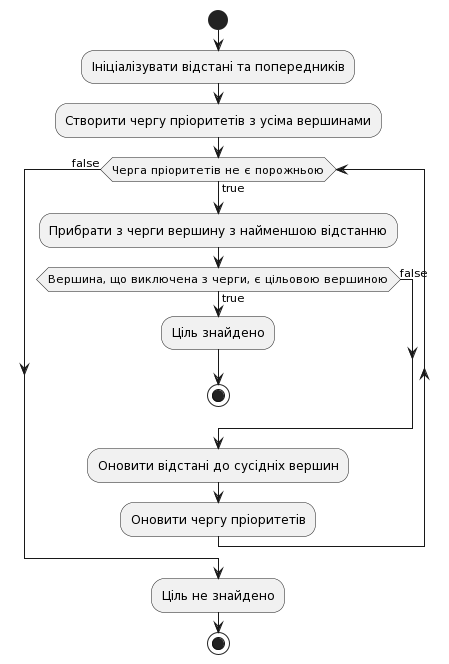
\includegraphics[scale=0.7]{content/chapters/2-implementation-methods/assets/img/dijkstras_algorithm.png}
    \caption{Блок-схема алгоритму Дейкстри}
    \label{fig:dijkstras}
\end{figure}

Переваги:
\begin{itemize}
    \item Гарантує знаходження найкоротшого шляху у зваженому графі з невід'ємними вагами ребер.
    \item Це відносно простий і зрозумілий алгоритм, що робить його гарним вибором для навчальних цілей.
    \item Його можна використовувати в широкому спектрі застосувань, від маршрутизації в комп'ютерних мережах до пошуку найкоротшого шляху в транспортних мережах.
    \item Він може обробляти графи з декількома шляхами однакової ваги, на відміну від деяких інших алгоритмів, які можуть працювати з такими випадками некоректно.
\end{itemize}

Недоліки:
\begin{itemize}
    \item Не працює коректно з від'ємними вагами ребер, оскільки може застрягти у нескінченному циклі.
    \item Може бути повільним на великих графах, особливо якщо черга пріоритетів, яка використовується для реалізації, не є ефективною.
    \item Він може бути не найкращим вибором для певних типів графів, наприклад, графів з високим ступенем зв'язності або графів з великою кількістю циклів.
    \item Він не обробляє графи з декількома найкоротшими шляхами між однією і тією ж парою вершин.
\end{itemize}
